

%\documentclass[pra,twocolumn,epsfig,rotate,superscriptaddress,showpacs]{revtex4}


% \mathcal{u}se only LaTeX2e, calling the article.cls class and 12-point type.

\documentclass[prl,onecolumn]{revtex4-1}
\usepackage{graphicx}
\usepackage{epsfig}
\usepackage{epsf}
\usepackage{amssymb}
\usepackage{amsmath}
\usepackage{amsthm}
\usepackage{multirow}
\usepackage{hyperref}

\usepackage{tabu} % table macro

\usepackage[framed,numbered]{matlab-prettifier}
\let\ph\snippetPlaceholder
\lstset
{
  style = Matlab-editor,
  escapechar      = ",
}

\renewcommand{\familydefault}{\sfdefault}  %% arial font
% \usepackage{times} %% times new roman font

\newcommand{\bra}[1]{\langle #1|}
\newcommand{\ket}[1]{|#1\rangle}
\newcommand{\dir}{$\backslash$}
\newcommand{\be}{\begin{equation}}
\newcommand{\ee}{\end{equation}}
\newcommand{\bea}{\begin{eqnarray}}
\newcommand{\eea}{\end{eqnarray}}
\newcommand{\Fig}[1]{Fig.\,\ref{#1}}
\newcommand{\Eq}[1]{Eq.\,(\ref{#1})}
\newcommand{\la}{\langle}
\newcommand{\ra}{\rangle}
\newcommand{\nl}{\nonumber \\}
%\usepackage[usenames]{color}
%\definecolor{Red}{rgb}{1,0,0}
%\definecolor{Blue}{rgb}{0,0,1}




\setlength{\parindent}{0pt} % no incident
%\renewcommand{\baselinestretch}{1.2} % space between two lines
\setlength{\parskip}{6\lineskip} % space between two paragraphs

%%%%%%%%%%%%%%%%% END OF PREAMBLE %%%%%%%%%%%%%%%%



\begin{document}

% Include your paper's title here
\title{Notes on the 12 qubit PPS}
\author{Dawei Lu}

\begin{abstract}
Notes about the problems in the 12 qubit PPS preparation, including Matlab codes and Experiments.
\end{abstract}
\today

\maketitle

\section{Dec 12, 2014}

Calculating the state to state GRAPE on Ordi2. In pulsefinder folder. paramsfile is 'twqubit\_subS2S.m', and the output file is 'twqubit\_7zto12z'.

The GRAPE is to evolve ZZZZZZZIIIII to ZZZZZZZZZZZZ. As the couplings between nearest-neighbored C and H are about 150Hz. I set the GRAPE

\begin{lstlisting}
% Number of timesteps
params.plength = 400;

% Length of each time step
params.timestep = 10e-6;

params.subsystem{1} = [1 2 3 9 10 11];
params.subsystem{2} = [4 5 6 7 8 12];
params.subsys_weight = [6 6];

% Input and goal states for state to state
params.rhoin = mkstate('+1ZZZZZZZIIIII',1);
params.rhogoal = mkstate('+1ZZZZZZZZZZZZ',1);

% Allow Zfreedom or not
params.Zfreedomflag = 1;
\end{lstlisting}

The fidelity keeps 0 all the time. Guess the reason is 'Zfreedom'. Set 'params.Zfreedomflag = 0;'. However, still 0.

Annie said maybe due to the length. Her SWAP gate requires 8ms, so I changed 'params.plength = 800;'. But for with or without Zfreedom, fidelity is still 0.

Check if some of my GRAPE settings are wrong. try to repeat Annie's SWAP gate calculation.

\begin{lstlisting}
% Number of timesteps
params.plength = 800;

% Length of each time step
params.timestep = 10e-6;

params.subsystem{1} = [1 2 3 9 10 11];
params.subsystem{2} = [4 5 6 7 8 12];
params.subsys_weight = [6 6];

% Input and goal states for state to state
params.rhoin = mkstate('+1IIIIIIIZIIII+1IIIIIIIIZIII+1IIIIIIIIIZII+1IIIIIIIIIIZI+1IIIIIIIIIIIZ',1);
params.rhogoal = mkstate('+1IIIIIIIZIIII+1IIIIIIIIZIII+1IIIIIIIIIZII+1IIIIIIIIIIZI+1IIIIIIZIIIIZ',1);

% Allow Zfreedom or not
params.Zfreedomflag = 0;
\end{lstlisting}

The outputfile is 'twqubit\_SWAPC7H5'. And the fidelity is already over 98\%. Then I changed 'params.Zfreedomflag = 1;', and the fidelity is over 95\% after 30 iterations. Much slower than the no Zfreedom case. Maybe due to different initial guesses.

\newpage

\section{Dec 15, 2014}

Generate all $\pi/2$ and $\pi$ pulses for the 7 Carbons, with the Calibration = 25KHz. $\pi/2$ pulses are 1ms length and 100 steps, and $\pi$ pulses are 2ms length and 200 steps. Generating Code in 'twqubit\_shape.m'

\begin{lstlisting}
for ii = 1:7
loadfile = ['twqubit_C', num2str(ii), '180', '.mat'];
eval(['load ', loadfile]);
filename1 = ['twqubit_C', num2str(ii), '180_C_25000.txt'];
filename2 = ['twqubit_C', num2str(ii), '180_H_25000.txt'];
make_bruker_shape(pulses{1}, 25000, filename1,1);
make_bruker_shape(pulses{1}, 25000, filename2,2);
end
\end{lstlisting}

The pulses are saved in Ordi2 '\dir pulsefinder\dir 12 Qubit\dir' with the names such as\\
'twqubit\_C590\_C\_25000.txt'.

I checked all the fidelities of the $\pi/2$ pulses in the folder '\dir pulseexam\_12qubit\dir C\_rotations\dir check\_grape.m'. The code is

\begin{lstlisting}
load Para.mat
load twpauliX_full.mat
load twpauliY_full.mat

%% Check all 90 rotations
%% Parameters for the GRAPE pulse
for spin_number = 1:7
Name1 = ['twqubit_C', num2str(spin_number), '90_C_25000.txt'];
Name2 = ['twqubit_C', num2str(spin_number), '90_H_25000.txt'];
Amplitude = 25000;
Time = 1e-3;
Length = 100;
dt = Time/Length;
FirstLine = 19; % the first line which contains the information of power and phase

Output1 = 'test1';
Output2 = 'test2';

[power1,phase1]=dataout(Name1,Output1,FirstLine,Length);
[power2,phase2]=dataout(Name2,Output2,FirstLine,Length);
%% Check
X_C = 0; Y_C = 0;
for jj = 1:7
    X_C = X_C + KIx{jj};
    Y_C = Y_C + KIy{jj};
end

X_H = 0; Y_H = 0;
for jj = 8:12
    X_H = X_H + KIx{jj};
    Y_H = Y_H + KIy{jj};
end


U = eye(2^12);
U = U*expm(-i*H*4e-6);
for ii = 1:Length
    Hext = 2*pi*(Amplitude*power1(ii)/100)*(X_C*cos(phase1(ii)/360*2*pi)-Y_C*sin(phase1(ii)/360*2*pi))+2*pi*(Amplitude*power2(ii)/100)*(X_H*cos(phase2(ii)/360*2*pi)-Y_H*sin(phase2(ii)/360*2*pi));
    U = expm(-i*(Hext+H)*dt)*U;
end
U = U*expm(-i*H*4e-6);

Utar = expm(-i*KIx{spin_number}*pi/2);

% Fidelity = ['Fidelity_C', num2str(spin_number), '90'];
% eval(['Fidelity_C', num2str(spin_number), '90 = abs(trace(U*Utar'))/2^12']);
Fidelity = abs(trace(U*Utar'))/2^12

savefile = ['twqubit_C', num2str(spin_number), '90_Ufid.mat'];
save (savefile, 'U', 'Fidelity');

end
\end{lstlisting}

Unitaries and Fidelities of the pulses will both be saved in 'twqubit\_C590\_Ufid.mat', so they can be called for further calculations in the PPS simulation. Wait for the results.

\newpage
\section{Dec 16, 2014}
Combine pulses in the PPS preparation into big shape files, which should be easy for calibrations and pulsefixing.

The code is in the SVN server for Matlab named '\dir Twqubit\dir pulse\_combine.m'.

First read all the powers and phases for the $\pi/2$ and $\pi$ rotations.

\begin{lstlisting}
for spin_number = 1:7
       Name1 = ['twqubit_C', num2str(spin_number), '90_C_25000.txt'];
       Name2 = ['twqubit_C', num2str(spin_number), '90_H_25000.txt'];
       [power1,phase1]=dataout(Name1,Output1,FirstLine,Length_90);
       [power2,phase2]=dataout(Name2,Output2,FirstLine,Length_90);
       eval(['power_C', num2str(spin_number), '90_C = power1;']); eval(['phase_C', num2str(spin_number), '90_C = phase1;']);
       eval(['power_H', num2str(spin_number), '90_H = power2;']); eval(['phase_H', num2str(spin_number), '90_H = phase2;']);
end

for spin_number = 1:7
       Name1 = ['twqubit_C', num2str(spin_number), '180_C_25000.txt'];
       Name2 = ['twqubit_C', num2str(spin_number), '180_H_25000.txt'];
       [power1,phase1]=dataout(Name1,Output1,FirstLine,Length_180);
       [power2,phase2]=dataout(Name2,Output2,FirstLine,Length_180);
       eval(['power_C', num2str(spin_number), '180_C = power1;']); eval(['phase_C', num2str(spin_number), '180_C = phase1;']);
       eval(['power_H', num2str(spin_number), '180_H = power2;']); eval(['phase_H', num2str(spin_number), '180_H = phase2;']);
end
\end{lstlisting}

Then combine them with the free evolutions. Here I set the time step dt = 10us.

\begin{lstlisting}
%% From Z7 to Z24567
step_27 = round(1/(4*Para(2,7))/dt);
step_67_27 = round((1/(4*Para(6,7))-1/(4*Para(2,7)))/dt);
step_47_67 = round((1/(4*Para(4,7))-1/(4*Para(6,7)))/dt);
step_57_47 = round((1/(4*Para(5,7))-1/(4*Para(4,7)))/dt);
step_57 = round((1/(4*Para(5,7)))/dt);

power_encoding1_C = [power_C790_C; zeros(step_27,1);power_C2180_C; zeros(step_67_27,1); power_C6180_C; zeros(step_47_67,1);power_C4180_C; zeros(step_57_47,1);...
                                  power_C5180_C; power_C7180_C; zeros(step_57,1);power_C790_C]*Calibration/Calibration_old;
phase_encoding1_C = [phase_C790_C; zeros(step_27,1);phase_C2180_C; zeros(step_67_27,1); phase_C6180_C; zeros(step_47_67,1);phase_C4180_C; zeros(step_57_47,1);...
                                  phase_C5180_C; phase_C7180_C; zeros(step_57,1);mod((phase_C790_C+90),360)];
power_encoding1_H = [power_H790_H; zeros(step_27,1);power_H2180_H; zeros(step_67_27,1); power_H6180_H; zeros(step_47_67,1);power_H4180_H; zeros(step_57_47,1);...
                                  power_H5180_H; power_H7180_H; zeros(step_57,1);power_H790_H]*Calibration/Calibration_old;
phase_encoding1_H = [phase_H790_H; zeros(step_27,1);phase_H2180_H; zeros(step_67_27,1); phase_H6180_H; zeros(step_47_67,1);phase_H4180_H; zeros(step_57_47,1);...
                                  phase_H5180_H; phase_H7180_H; zeros(step_57,1);mod((phase_H790_H+90),360)];

total_time_encoding1 = length(power_encoding1_C)*dt;

outputfile = 'twqubit_encoding1_C';
shpfile = fopen(outputfile,'w');
    fprintf(shpfile,'##TITLE= %s\n',outputfile);
    fprintf(shpfile,'##JCAMP-DX= 5.00 Bruker JCAMP library\n');
    fprintf(shpfile,'##DATA TYPE= Shape Data\n');
    fprintf(shpfile,'##ORIGIN= Dawei''s GRAPE Pulses \n');
    fprintf(shpfile,'##OWNER= Dawei\n');
    fprintf(shpfile,'##DATE= %s\n',date);
    time = clock;
    fprintf(shpfile,'##TIME= %d:%d\n',fix(time(4)),fix(time(5)));
    fprintf(shpfile,'##MINX= %7.6e\n',min(power_encoding1_C));
    fprintf(shpfile,'##MAXX= %7.6e\n',max(power_encoding1_C));
    fprintf(shpfile,'##MINY= %7.6e\n',min(phase_encoding1_C));
    fprintf(shpfile,'##MAXY= %7.6e\n',max(phase_encoding1_C));
    fprintf(shpfile,'##$SHAPE_EXMODE= None\n');
    fprintf(shpfile,'##$SHAPE_TOTROT= %7.6e\n',90);
    fprintf(shpfile,'##$SHAPE_BWFAC= %7.6e\n',1);
    fprintf(shpfile,'##$SHAPE_INTEGFAC= %7.6e\n',1);
    fprintf(shpfile,'##$SHAPE_MODE= 1\n');
    fprintf(shpfile, '##PULSE_WIDTH= %d\n',total_time_encoding1);
    fprintf(shpfile, '##Calibration_Power= %d\n',Calibration);
    fprintf(shpfile,'##NPOINTS= %d\n',length(power_encoding1_C));
    fprintf(shpfile,'##XYPOINTS= (XY..XY)\n');

for ii = 1:length(power_encoding1_C)
    fprintf(shpfile,'  %7.6e,  %7.6e\n',power_encoding1_C(ii),phase_encoding1_C(ii));
end

    fprintf(shpfile,'##END=\n');

outputfile = 'twqubit_encoding1_H';
shpfile = fopen(outputfile,'w');
    fprintf(shpfile,'##TITLE= %s\n',outputfile);
    fprintf(shpfile,'##JCAMP-DX= 5.00 Bruker JCAMP library\n');
    fprintf(shpfile,'##DATA TYPE= Shape Data\n');
    fprintf(shpfile,'##ORIGIN= Dawei''s GRAPE Pulses \n');
    fprintf(shpfile,'##OWNER= Dawei\n');
    fprintf(shpfile,'##DATE= %s\n',date);
    time = clock;
    fprintf(shpfile,'##TIME= %d:%d\n',fix(time(4)),fix(time(5)));
    fprintf(shpfile,'##MINX= %7.6e\n',min(power_encoding1_H));
    fprintf(shpfile,'##MAXX= %7.6e\n',max(power_encoding1_H));
    fprintf(shpfile,'##MINY= %7.6e\n',min(phase_encoding1_H));
    fprintf(shpfile,'##MAXY= %7.6e\n',max(phase_encoding1_H));
    fprintf(shpfile,'##$SHAPE_EXMODE= None\n');
    fprintf(shpfile,'##$SHAPE_TOTROT= %7.6e\n',90);
    fprintf(shpfile,'##$SHAPE_BWFAC= %7.6e\n',1);
    fprintf(shpfile,'##$SHAPE_INTEGFAC= %7.6e\n',1);
    fprintf(shpfile,'##$SHAPE_MODE= 1\n');
    fprintf(shpfile, '##PULSE_WIDTH= %d\n',total_time_encoding1);
    fprintf(shpfile, '##Calibration_Power= %d\n',Calibration);
    fprintf(shpfile,'##NPOINTS= %d\n',length(power_encoding1_H));
    fprintf(shpfile,'##XYPOINTS= (XY..XY)\n');

for ii = 1:length(power_encoding1_H)
    fprintf(shpfile,'  %7.6e,  %7.6e\n',power_encoding1_H(ii),phase_encoding1_H(ii));
end

    fprintf(shpfile,'##END=\n');
\end{lstlisting}

The two output files are 'twqubit\_encoding1\_C' and 'twqubit\_encoding1\_H'. The calibrations are 25000Hz.

\newpage
\section{Dec 17, 2014}

All fidelities of $\pi/2$ pulses are done! The folder is '\dir pulseexam\_12qubit\dir C\_rotations\dir'. Use 'check\_power.m' to check the maximal powers for C and H channel.

\begin{table}[hbtp]
\begin{tabular} {c||c|c|c|c}
  \hline
  Rotation & Fidelity & File & MaxPower C & MaxPower H\\
  \hline
  % after \\: \hline or \cline{col1-col2} \cline{col3-col4} ...
  $R_x^1(\pi/2)$ & 0.9838 & twqubit\_C190\_Ufid.mat & 56.0\%, 14000Hz & 22.3\%, 5557Hz\\
  $R_x^2(\pi/2)$ & 0.9758 & twqubit\_C290\_Ufid.mat & 41.7\%, 10422Hz & 23.5\%, 5878Hz\\
  $R_x^3(\pi/2)$ & 0.9647 & twqubit\_C390\_Ufid.mat & 31.9\%, 7979.0Hz & 22.3\%, 5568Hz\\
  $R_x^4(\pi/2)$ & 0.9801 & twqubit\_C490\_Ufid.mat & 31.6\%, 7892.0Hz & 23.8\%, 5954Hz\\
  $R_x^5(\pi/2)$ & 0.9936 & twqubit\_C590\_Ufid.mat & 56.1\%, 14033Hz & 30.7\%, 7678Hz\\
  $R_x^6(\pi/2)$ & 0.9683 & twqubit\_C690\_Ufid.mat & 57.3\%, 14333Hz & 34.4\%, 8595Hz\\
  $R_x^7(\pi/2)$ & 0.9857 & twqubit\_C790\_Ufid.mat & 43.7\%, 10925Hz & 24.8\%, 6207Hz\\
  \hline
  \hline
  $R_x^1(\pi)$ & 0.9699 & twqubit\_C1180\_Ufid.mat & 62.6\%, 15655Hz & 34.9\%, 8726Hz\\
  $R_x^2(\pi)$ & 0.9537 & twqubit\_C2180\_Ufid.mat & 51.1\%, 12783Hz & 32.4\%, 8094Hz\\
  $R_x^3(\pi)$ & 0.9330 & twqubit\_C3180\_Ufid.mat & 37.4\%, 9350.0Hz & 24.0\%, 5997Hz\\
  $R_x^4(\pi)$ & 0.9639 & twqubit\_C4180\_Ufid.mat & 45.1\%, 11268Hz & 20.4\%, 5108Hz\\
  $R_x^5(\pi)$ & 0.9904 & twqubit\_C5180\_Ufid.mat & 67.6\%, 16895Hz & 31.1\%, 7782Hz\\
  $R_x^6(\pi)$ & 0.9393 & twqubit\_C6180\_Ufid.mat & 71.8\%, 17948Hz & 33.6\%, 8396Hz\\
  $R_x^7(\pi)$ & 0.9743 & twqubit\_C7180\_Ufid.mat & 51.0\%, 12759Hz & 32.1\%, 8022Hz\\
  \hline
\end{tabular}
\end{table}

For $\pi$ pulses, the maximal power of C5 exceeds 100\% so it cannot be used. Check if we can generate $\pi$ pulses by combining two $\pi/2$ pulses. A potential problem is when calculating the GRAPE, we have considered the 4us free evolutions in the beginning and in the end. If we combine, we will have an unwanted 8us free evolution in the middle of the new $\pi$ pulse.

Use 'combine90to180' to check the $\pi$ pulse fidelity. They are very bad actually. All of them are just 0.75~0.76 in fidelity.

So I run 'check\_grape.m' to check the fidelities of the $\pi$ pulses. Only from C1 to C4, as C5 has exceeds the power limit 25000Hz.

\newpage
\section{Dec 22, 2014}

Got 4 GRAPE pulses for encoding. The folder is '\dir pulseexam\_12qubit\dir C\_rotations\dir'. The fidelities are in calculation on Ordi2.

\begin{table}[hbtp]
\begin{tabular} {c||c|c|c|c}
  \hline
  Rotation & Fidelity & File & MaxPower C & MaxPower H\\
  \hline
  % after \\: \hline or \cline{col1-col2} \cline{col3-col4} ...
  $R_x^{5,7}(\pi)$ & 0.9667 & twqubit\_C57180\_Ufid.mat & 32.3\%, 8072.5Hz & 24.2\%, 6049Hz\\
  $R_x^{2,3}(\pi)$ & 0.8908 & twqubit\_C23180\_Ufid.mat & 32.4\%, 8101.5Hz & 22.8\%, 5701Hz\\
  $R_x^{2,3,4,7}(\pi/2)$ & 0.9156 & twqubit\_C234790\_Ufid.mat & 37.4\%, 9358.3Hz & 28.9\%, 7213Hz\\
  $R_x^{1,5,6}(\pi)$ & 0.9055 & twqubit\_C156180\_Ufid.mat & 32.2\%, 8039.7Hz & 20.3\%, 5086Hz\\
  \hline
\end{tabular}
\end{table}

Have to recalculate many $\pi$ pulses.

\newpage
\section{Dec 23, 2014}

Got $\pi$ pulse on C6. Combine two $\pi/2$ pulses as the initial guess, with the fidelity 0.75, and then search the optimal $\pi$ pulse. The convergence speed is very fast, which means initial guess is indeed very important in 12 qubits.

Now C2, C3, C5, C7 $\pi$ pulses are in calculation, with the initial guess.

\newpage
\section{Feb 05, 2015}

C2, C3, C5, C7 $\pi$ pulses are all finished, and the update is in the Section Dec 17, 2014.

Also submitted the last pulse for the Encoding. From the PPS.m file in folder 'Twqubit'
\begin{lstlisting}
%Phase Correction
U7 = R(gop(2,X),90)*R(gop(2,-Z),360*(Para(2,2)-20696)*1/2/148.5)*...
R(gop(3,-Y),90)*R(gop(3,-Z),360*(Para(3,3)-20696)*1/2/148.5)*...
R(gop(4,X),90)*R(gop(4,-Z),360*(Para(4,4)-20696)*1/2/148.5)*...
R(gop(7,X),90)*R(gop(7,-Z),360*(Para(7,7)-20696)*1/2/148.5);
\end{lstlisting}

And the operator is in 'twqubit\_sub\_234790\_and\_phasecorrection.m'
\begin{lstlisting}
params.Uwant = expm(-1i*(90*pi/180)/2*full(mkstate('+1IXIIIIIIIIII-1IIYIIIIIIIII+1IIIXIIIIIIII+1IIIIIIXIIIII',0)))*...
expm(-1i*((8778.95-20696)*1/2/148.5*360*pi/180)/2*full(mkstate('-1IZIIIIIIIIII',0)))*...
expm(-1i*((6245.16675-20696)*1/2/148.5*360*pi/180)/2*full(mkstate('-1IIZIIIIIIIII',0)))*...
expm(-1i*((10333.55-20696)*1/2/148.5*360*pi/180)/2*full(mkstate('-1IIIZIIIIIIII',0)))*...
expm(-1i*((11928.21998-20696)*1/2/148.5*360*pi/180)/2*full(mkstate('-1IIIIIIZIIIII',0)));
\end{lstlisting}

\newpage
\section{Feb 06, 2015}

The pulse 'twqubit\_sub\_234790\_and\_phasecorrection.m' which is the last piece of the encoding was found!

All $\pi$ pulses are found. The lowest is 0.9330 for C3 and the highest is 0.9904 for C5. Now is calculating the fidelity of the last piece in Encoding
'twqubit\_C234790withPC\_Ufid.mat'. Will combine all of the pulses in Encoding and check again after this calculation.

The last piece 'twqubit\_C234790withPC\_Ufid.mat' has been checked. The fidelity is 0.9164.

\newpage
\section{Feb 12, 2015}

When combining all pulses into a large shape file, one has to know how to change a shape for X rotation to Y rotation. It should be a $\pi/2$ phase difference for every segment in the shape. I am going to check it.

The checking uses 4-qubit Crotonic in the folder 'F:\dir matlab\dir pulseexam\_7qubit\dir 4 qubit pulse check'. The target unitary is $R_x^1(\pi/2)$, and the pulse is 'Croton\_90x1.txt' with length 1ms, 500 segments and amplitude 6000Hz.

When compared with $R_x^1(\pi/2)$, the fidelity is 0.9996. Then I changed the target to $R_y^1(\pi/2)$ with the GRAPE pulse unchanged. The fidelity goes to 0.4998 which is reasonable.

In order to produce a $R_y^1(\pi/2)$ from the original X rotation pulse, I added 90 to all phases in all segments. However, the fidelity goes to almost 0. Again all phases are reduced by 90, and this time the fidelity is 0.9996, which is what we want!

Conclusion: If you want to realize a Y rotation based on a X rotation pulse, just change the phase to phase-90 in each segment, and mod by 360 for the spectrometer.
\begin{lstlisting}
phase = phase - 90;
phase = mod(phase, 360);
\end{lstlisting}
I wrote a program 'grape\_phase' to generate the new phase in the folder 'F:\dir matlab\dir pulseexam\_7qubit\dir'. Used in this manner  'phase\_new = grape\_phase( phase, initial\_phase, end\_phase)', where the initial\_phase and end\_phase can be X, Y, -X, or -Y.

The way to get the new operator is through the equation $R_z(\theta) = XR_y(\theta)\bar{X}$. If you know the unitary $U_x$ of the X rotation pulse, and when you are realizing Y pulse from that one, the new unitary $U_y$ is thus
\be
U_y = R_z(\pi/2)U_xR_z(-\pi/2);
\ee

Generated the first encoding part, which will evolve Z7 to Z24567. The files 'twqubit\_encoding1\_C' and 'twqubit\_encoding1\_H' are in Ordi2 '\dir pulseexam\_12qubit'. The total length is 32.98ms. Next I have to check whether the final state after this pulse will be Z24567 or not. So 'check\_encoding.m' is written. The directory is Ordi2 '\dir pulseexam\_12qubit'. This function will load all necessary .mat files to get the unitaries and calculate the final state based on these unitaries from Z7.

The final fidelity is 0.9832 (the same for with or without gradient) for Z24567. Two files 'U\_encoding1.mat' and 'rho\_encoding1.mat'. Now go on to the second Encoding part.

The fidelity for the second Encoding part is -0.9692 (the same for with or without gradient) for Z1234567. Two files 'twqubit\_encoding2\_C' and 'twqubit\_encoding2\_H' are in Ordi2 '\dir pulseexam\_12qubit'. The total length is 21.29ms. Then the last piece in Encoding!

The fidelity for the third Encoding part is -0.9160 (the same for with or without gradient) for Z123456789101112. Two files 'twqubit\_encoding3\_C' and 'twqubit\_encoding3\_H' are in Ordi2 '\dir pulseexam\_12qubit'. The total length is 7.36ms.

\textbf{Update on Mar 04}: In the last code, the free evolution time is not the integer times of 10us, but it should be. So the function 'F.m' is modified as
\begin{lstlisting}
function F=F(Hamiltonian, time)
F=diag(exp(diag(-i*Hamiltonian*10e-6*round(time/10e-6))),0);
\end{lstlisting}
And all the fidelities are recalculated. They are 0.9831 for Encoding 1,  -0.9717 for Encoding 2, -0.9124 for Encoding 3.

\newpage
\section{Feb 18, 2015}

Running the two pulses. One is 'twqubit\_all90.m' which is used for phase cycling, and the other one is 'twqubit\_all90butC7.m' used for the polarization crush in the beginning.
The fidelities are obtained!
\begin{table}[hbtp]
\begin{tabular} {c||c|c|c|c|c}
  \hline
  Rotation & Length & Fidelity & File & MaxPower C & MaxPower H\\
  \hline
  % after \\: \hline or \cline{col1-col2} \cline{col3-col4} ...
  $R_x^{1-12}(\pi/2)$ & 1ms & 0.8738 & twqubit\_all90\_Ufid.mat & 27.8\%, 6956.6Hz & 30.4\%, 7594Hz\\
  $R_x^{1-6,8-12}(\pi/2)$ & 1ms & 0.8849 & twqubit\_all90butC7\_Ufid.mat & 24.5\%, 6134.9Hz & 25.0\%, 6239Hz\\
  \hline
\end{tabular}
\end{table}

\newpage
\section{Feb 23, 2015}

Running all 6 pulses for the decoding part. Got 2, 3, 5 and 6! But the first pulse 'twqubit\_C2347andH180.m' has to be recalculated.

Then check all the fidelities for pulse 2, 3, 5 and 6 first.

\newpage
\section{Mar 3, 2015}

All 6 pulses in decoding have been checked. To my surprise some fidelities are pretty, such as the fidelity of $R_x^{2,3,4,5,6}(\pi)$ is only 0.8058. Anyway, it is better to check the state fidelity right away.

\begin{table}[hbtp]
\begin{tabular} {c||c|c|c|c|c}
  \hline
  Rotation & Length & Fidelity & File & MaxPower C & MaxPower H\\
  \hline
  % after \\: \hline or \cline{col1-col2} \cline{col3-col4} ...
  $R_x^{2,3,4,7-12}(\pi)$ & 2ms & 0.8424 & twqubit\_C2347andH180\_Ufid.mat & 61.6\%, 15400Hz & 52.2\%, 13039Hz\\
  $R_x^{1,3,4,6}(\pi/2)R_{-y}^{8-12}(\pi/2)$ & 1ms & 0.9080 & twqubit\_C134690andH90\_Ufid.mat & 24.8\%, 6203.2Hz & 22.1\%, 5529Hz\\
  $R_x^{2,3,4,5,6}(\pi)$ & 2ms & 0.8058 & twqubit\_C23456180\_Ufid.mat & 37.8\%, 9438.2Hz & 23.0\%, 5746Hz\\
  $R_{-y}^{1,3,4,6}(\pi/2)R_{x}^{2}(\pi/2)R_{-z}^{1}(\frac{1}{2J23}-\frac{1}{2J12})$ & 1ms & 0.8881 & twqubit\_C1234690withPC\_Ufid.mat & 21.2\%, 5310.9Hz & 22.9\%, 5724Hz\\
  $R_x^{2,7}(\pi)$ & 2ms & 0.9306 & twqubit\_C27180\_Ufid.mat & 29.1\%, 7285.3Hz & 21.7\%, 5414Hz\\
  $R_{-y}^{2}(\pi/2)R_{x}^{5}(\pi/2)$ & 1ms & 0.9728 & twqubit\_C2Y5X90\_Ufid.mat & 59.2\%, 14795Hz & 40.9\%, 10232Hz\\
  \hline
\end{tabular}
\end{table}

\newpage
\section{Mar 4, 2015: Re-Check the PPS Circuit in Simulation}

I found the decoding part can be simplified. Check it in Matlab.

All the files are saved in Ordi2 '\dir twqubit\dir'. For the encoding which consists of three parts, the fidelities have been checked before.
\begin{table}[hbtp]
\caption{Encoding in 12-qubit PPS}
\begin{tabular} {c||c|c|c}
  \hline
  Target State & State Fidelity & Density Matrix & Unitary Operator\\
  \hline
  % after \\: \hline or \cline{col1-col2} \cline{col3-col4} ...
  IZIZZZXIIIII & 1.0000 & rho\_encoding1.mat & U\_encoding1.mat\\
  ZXZZZZZIIIII & -1.0000 & rho\_encoding2.mat & U\_encoding2.mat\\
  ZZZZZZZZZZZZ & -0.9500 & rho\_encoding3.mat & U\_encoding3.mat\\
  \hline
\end{tabular}
\end{table}

For the phase cycling it has been done too.
\begin{table}[hbtp]
\caption{Phase Cycling in 12-qubit PPS}
\begin{tabular} {c||c|c|c}
  \hline
  Target State & State Fidelity & Density Matrix & Unitary Operator\\
  \hline
  % after \\: \hline or \cline{col1-col2} \cline{col3-col4} ...
  $\ket{00...0}\bra{00...0} + \ket{11...1}\bra{11...1}$ & 0.9511 & rho\_phasecycling.mat & NAN\\
  \hline
\end{tabular}
\end{table}

For the decoding part, the simulation is as follows.
\begin{table}[hbtp]
\caption{Decoding in 12-qubit PPS}
\begin{tabular} {c||c|c|c}
  \hline
  Target State & State Fidelity & Density Matrix & Unitary Operator\\
  \hline
  % after \\: \hline or \cline{col1-col2} \cline{col3-col4} ...
  $\begin{array}{c}
     A_1A_5A_6 \ket{+---++-00000}+ \\
     A_1'A_5'A_6' \ket{-+++--+00000}
   \end{array}
  $ & 0.8717 & rho\_decoding1.mat & U\_decoding1.mat\\
  \hline
    $\begin{array}{c}
     A_1A_5A_6A_7 \ket{0+00-0-00000}+ \\
     A_1'A_5'A_6'A_7' \ket{0-00+0+00000}
   \end{array}
  $ & 0.8570 & rho\_decoding2.mat & U\_decoding2.mat\\
  \hline
  $\begin{array}{c}
     A_1A_5A_6A_7A_5^{new} \ket{000000-00000}+ \\
     A_1'A_5'A_6'A_7'A_5^{new'} \ket{000000+00000}
   \end{array}
  $ & 0.8570 & rho\_decoding3.mat & U\_decoding3.mat\\
  \hline
\end{tabular}
\end{table}

A$_1$, A$_5$ and A$_6$ are phases produced by the chemical shift evolutions of C1, C5 and C6 during $1/2\text{J}_{\text{C7H5}}$. A$_7$ is the phase by the chemical shift evolution of C7 (\textbf{Note: C7 is x-iy so the phase is the conjugate}) during $1/2\text{J}_{\text{C2C3}}$, and the coupling evolutions between C7 and all protons. A$_5^{new}$ is the phase of C5 again in $1/2\text{J}_{\text{27}}$, including the chemical shift evolution and coupling evolutions (J25 and J57 are switched off). So the phases are
\bea
A_1 & = &cos(2\pi(\omega_1-O_1)/2\text{J}_{\text{C7H5}})-isin(2\pi(\omega_1-O_1)/2\text{J}_{\text{C7H5}}), \\ \nonumber
A_5 & = &cos(2\pi(\omega_5-O_1)/2\text{J}_{\text{C7H5}})-isin(2\pi(\omega_5-O_1)/2\text{J}_{\text{C7H5}}), \\ \nonumber
A_6 & = &cos(2\pi(\omega_6-O_1)/2\text{J}_{\text{C7H5}})-isin(2\pi(\omega_6-O_1)/2\text{J}_{\text{C7H5}}), \\ \nonumber
A_7 & = &cos(2\pi(\omega_7-O_1)/2\text{J}_{\text{23}})+isin(2\pi(\omega_7-O_1)/2\text{J}_{\text{23}})* \\ \nonumber
&& \prod_{k=8}^{12} (cos(\pi\text{J}_{\text{7k}}/\text{J}_{\text{23}})+isin(\pi\text{J}_{\text{7k}}/\text{J}_{\text{23}})), \\ \nonumber
A_5^{new} & = &cos(2\pi(\omega_5-O_1)/2\text{J}_{\text{27}})+isin(2\pi(\omega_5-O_1)/2\text{J}_{\text{27}})* \\ \nonumber
&& \prod_{k\neq 2, 5, 7} (cos(\pi\text{J}_{\text{5k}}/\text{J}_{\text{27}})+isin(\pi\text{J}_{\text{5k}}/\text{J}_{\text{27}})) \\ \nonumber
\eea

When calculating the evolutions in the Decoding part, using the following equations (the evolution is 1/2J with two $\pi$ pulses inserted in the middle. \textbf{Note: without $\pi$ in the end})
\bea
(X+iY)\otimes(X+iZ) \longrightarrow (X-iY)\otimes(I+Z), \\ \nonumber
(X-iY)\otimes(X+iZ) \longrightarrow (X+iY)\otimes(I-Z), \\ \nonumber
(X+iY)\otimes(X-iZ) \longrightarrow (X+iY)\otimes(I-Z), \\ \nonumber
(X-iY)\otimes(X-iZ) \longrightarrow (X+iY)\otimes(I+Z).
\eea

\newpage
\section{Mar 10, 2015: Check the simulated spectra for the 12 qubit PPS circuit}

The final state 'rho\_decoding3.mat' includes a phase on C7. 'rho\_decoding3(1,33) = 0.1979 + 0.5728i', and I used a Z rotation $R_z^7(\theta)$ to rotate it into X. The rotating angle $\theta$ is 1.2381, and the element becomes 0.6060 after the rotation. Note 0.6060/0.7071 (the ideal value) = 0.8570 which is exactly the fidelity for the final state 'rho\_decoding3'. The new state is named 'rho\_12pps\_circuit', and is saved in Ordi2 '\dir twqubit\dir rho\_12pps\_circuit.mat'.

The simulation is implemented in Ordi2 '\dir NMR\dir Experiments\dir twqubit'. The main file is 'sim\_twqubit.m'.

Some settings:
o1\_C = 20696, o1\_H = 2894, td = 281684, swh = 30030.

The decoherence time is set in '\dir SRC\dir simulator\dir spectrumfast.m' and the value for C7 is chosen as 450ms.

1) For thermal, the spectrum file is saved in 'F:\dir matlab\_full\dir IQC\_simulation\dir PPS 12 qubit\dir sim\_thermal\_450ms.mat'.

2) For PPS of the circuit, copy 'rho\_12pps\_circuit.mat' to the folder '\dir SRC\dir simulator\dir' and change the function 'mkstate.m'. The spectrum file is saved in 'F:\dir matlab\_full\dir IQC\_simulation\dir PPS 12 qubit\dir sim\_pps\_obC7\_phasefixed.mat' (phase fixed means the final coherence is on X axis by applying a Z rotation).

The comparison (\textbf{Note the PPS data should be divided by 24}) is shown in the following Fig. \ref{spectra}.

\begin{figure}[htb]
\begin{center}
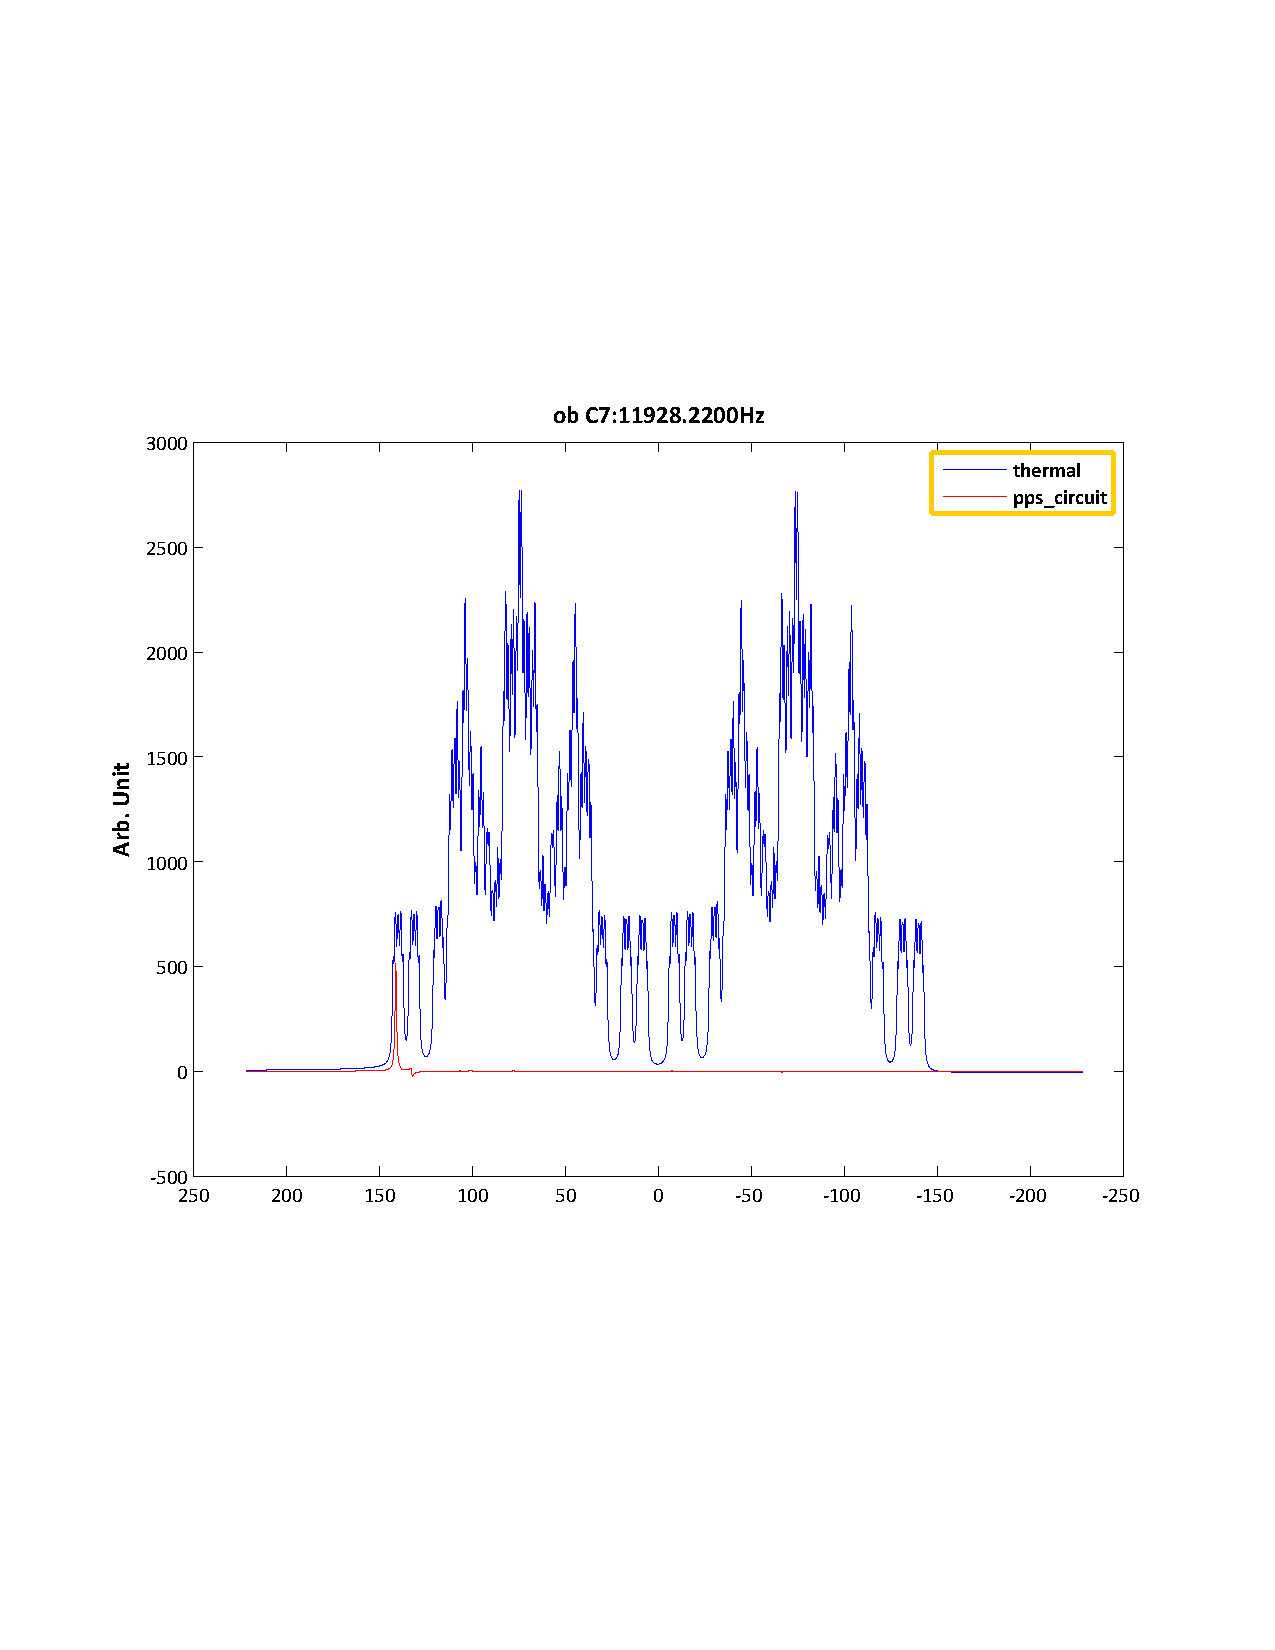
\includegraphics[width=\columnwidth]{thermal_and_pps_circuit.pdf}
\end{center}
\setlength{\abovecaptionskip}{-0.35cm}
\caption{\footnotesize{Comparison of the thermal and PPS produced by the circuit. }}\label{spectra}
\end{figure}

\newpage
\section{Mar 10, 2015: Check the simulated spectra for the 12 qubit PPS grape}

The unitaries for all rotations have been saved in Ordi2. So I only combined them with the free evolutions. \textbf{Note the time step is 10us, which means the free evolutions are integer times of 10us with the unwanted chemical shift refocusing (important!!!).}

Evolution times for every part.

Encoding1:
\begin{table}[hbtp]
\begin{tabular} {c||c|c|c|c|c|c}
  \hline
   Name & Total & $1/4\text{J}_{27}$ & $1/4\text{J}_{67}-1/4\text{J}_{27}$ & $1/4\text{J}_{47}-1/4\text{J}_{67}$ & $1/4\text{J}_{57}-1/4\text{J}_{47}$ & $1/4\text{J}_{57}$\\
  \hline
  Encoding1 & 32.98ms & 6670us & 560us & 1380us & 2880us & 11490us\\
  \hline
\end{tabular}
\end{table}

Encoding2:
\begin{table}[hbtp]
\begin{tabular} {c||c|c|c|c}
  \hline
   Name & Total & $1/4\text{J}_{12}$ & $1/4\text{J}_{23}-1/4\text{J}_{12}$ & $1/4\text{J}_{23}$\\
  \hline
  Encoding2 & 21.28ms & 4340us & 3300us & 7640us\\
  \hline
\end{tabular}
\end{table}

Encoding3:
\begin{table}[hbtp]
\begin{tabular} {c||c|c|c}
  \hline
   Name & Total & $1/4\text{J}_{\text{CH}}$ & $1/4\text{J}_{\text{CH}}$\\
  \hline
  Encoding3 & 7.36ms & 1680us & 1680us\\
  \hline
\end{tabular}
\end{table}

Decoding1:
\begin{table}[hbtp]
\begin{tabular} {c||c|c|c}
  \hline
   Name & Total & $1/4\text{J}_{\text{CH}}$ & $1/4\text{J}_{\text{CH}}$\\
  \hline
  Decoding1 & 7.36ms & 1680us & 1680us\\
  \hline
\end{tabular}
\end{table}

\newpage
\section{All Pulses for 12 qubits}

The saving folder is '\dir pulseexam\_12qubit\dir C\_rotations\dir'.

$\pi/2$ and $\pi$ rotations on every single spin.
\begin{table}[hbtp]
\begin{tabular} {c||c|c|c|c|c}
  \hline
  Rotation & Length & Fidelity & File & MaxPower C & MaxPower H\\
  \hline
  % after \\: \hline or \cline{col1-col2} \cline{col3-col4} ...
  $R_x^1(\pi/2)$ & 1ms & 0.9838 & twqubit\_C190\_Ufid.mat & 56.0\%, 14000Hz & 22.3\%, 5557Hz\\
  $R_x^2(\pi/2)$ & 1ms & 0.9758 & twqubit\_C290\_Ufid.mat & 41.7\%, 10422Hz & 23.5\%, 5878Hz\\
  $R_x^3(\pi/2)$ & 1ms & 0.9647 & twqubit\_C390\_Ufid.mat & 31.9\%, 7979.0Hz & 22.3\%, 5568Hz\\
  $R_x^4(\pi/2)$ & 1ms & 0.9801 & twqubit\_C490\_Ufid.mat & 31.6\%, 7892.0Hz & 23.8\%, 5954Hz\\
  $R_x^5(\pi/2)$ & 1ms & 0.9936 & twqubit\_C590\_Ufid.mat & 56.1\%, 14033Hz & 30.7\%, 7678Hz\\
  $R_x^6(\pi/2)$ & 1ms & 0.9683 & twqubit\_C690\_Ufid.mat & 57.3\%, 14333Hz & 34.4\%, 8595Hz\\
  $R_x^7(\pi/2)$ & 1ms & 0.9857 & twqubit\_C790\_Ufid.mat & 43.7\%, 10925Hz & 24.8\%, 6207Hz\\
  \hline
  \hline
  $R_x^1(\pi)$ & 2ms & 0.9699 & twqubit\_C1180\_Ufid.mat & 62.6\%, 15655Hz & 34.9\%, 8726Hz\\
  $R_x^2(\pi)$ & 2ms & 0.9537 & twqubit\_C2180\_Ufid.mat & 51.1\%, 12783Hz & 32.4\%, 8094Hz\\
  $R_x^3(\pi)$ & 2ms & 0.9330 & twqubit\_C3180\_Ufid.mat & 37.4\%, 9350.0Hz & 24.0\%, 5997Hz\\
  $R_x^4(\pi)$ & 2ms & 0.9639 & twqubit\_C4180\_Ufid.mat & 45.1\%, 11268Hz & 20.4\%, 5108Hz\\
  $R_x^5(\pi)$ & 2ms & 0.9904 & twqubit\_C5180\_Ufid.mat & 67.6\%, 16895Hz & 31.1\%, 7782Hz\\
  $R_x^6(\pi)$ & 2ms & 0.9393 & twqubit\_C6180\_Ufid.mat & 71.8\%, 17948Hz & 33.6\%, 8396Hz\\
  $R_x^7(\pi)$ & 2ms & 0.9743 & twqubit\_C7180\_Ufid.mat & 51.0\%, 12759Hz & 32.1\%, 8022Hz\\
  \hline
\end{tabular}
\end{table}

Pulses for the encoding part of PPS preparation.
\begin{table}[hbtp]
\begin{tabular} {c||c|c|c|c|c}
  \hline
  Rotation & Length & Fidelity & File & MaxPower C & MaxPower H\\
  \hline
  % after \\: \hline or \cline{col1-col2} \cline{col3-col4} ...
  $R_x^{5,7}(\pi)$ & 2ms & 0.9667 & twqubit\_C57180\_Ufid.mat & 32.3\%, 8072.5Hz & 24.2\%, 6049Hz\\
  $R_x^{2,3}(\pi)$ & 2ms & 0.8908 & twqubit\_C23180\_Ufid.mat & 32.4\%, 8101.5Hz & 22.8\%, 5701Hz\\
  $R_x^{2,3,4,7}(\pi/2)$ & 1ms & 0.9156 & twqubit\_C234790\_Ufid.mat & 37.4\%, 9358.3Hz & 28.9\%, 7213Hz\\
  $R_x^{1,5,6}(\pi)$ & 2ms & 0.9055 & twqubit\_C156180\_Ufid.mat & 32.2\%, 8039.7Hz & 20.3\%, 5086Hz\\
  $R_x^{2,4,7}(\pi/2)R_{-y}^{3}(\pi/2)R_{-z}^{i=2,3,4,7}((w_i-O_1)*1/2J_{CH})$ & 1ms & 0.9153 & twqubit\_C234790withPC\_Ufid.mat & 26.1\%, 6514.5Hz & 20.2\%, 5048Hz\\
  \hline
\end{tabular}
\end{table}

All 3 Encoding pulses in the saving folder '\dir pulseexam\_12qubit\dir'. The fidelities in the following table are state fidelities
\begin{table}[hbtp]
\begin{tabular} {c||c|c|c}
  \hline
  Files & Length & Target State & State Fidelity\\
  \hline
  % after \\: \hline or \cline{col1-col2} \cline{col3-col4} ...
  twqubit\_encoding1\_C, H & 32.98ms & IZIZZZZIIIII & 0.9831\\
  twqubit\_encoding2\_C, H & 21.28ms & ZZZZZZZIIIII & -0.9717\\
  twqubit\_encoding3\_C, H & 7.36 ms & ZZZZZZZZZZZZ & -0.9124\\
  \hline
\end{tabular}
\end{table}

\newpage
Pulses for polarization crush and phase cycling.
\begin{table}[hbtp]
\begin{tabular} {c||c|c|c|c|c}
  \hline
  Rotation & Length & Fidelity & File & MaxPower C & MaxPower H\\
  \hline
  % after \\: \hline or \cline{col1-col2} \cline{col3-col4} ...
  $R_x^{1-12}(\pi/2)$ & 1ms & 0.8738 & twqubit\_all90\_Ufid.mat & 27.8\%, 6956.6Hz & 30.4\%, 7594Hz\\
  $R_x^{1-6,8-12}(\pi/2)$ & 1ms & 0.8849 & twqubit\_all90butC7\_Ufid.mat & 24.5\%, 6134.9Hz & 25.0\%, 6239Hz\\
  \hline
\end{tabular}
\end{table}

Pulses for the decoding part of PPS preparation.
\begin{table}[hbtp]
\begin{tabular} {c||c|c|c|c|c}
  \hline
  Rotation & Length & Fidelity & File & MaxPower C & MaxPower H\\
  \hline
  % after \\: \hline or \cline{col1-col2} \cline{col3-col4} ...
  $R_x^{2,3,4,7-12}(\pi)$ & 2ms & 0.8424 & twqubit\_C2347andH180\_Ufid.mat & 61.6\%, 15400Hz & 52.2\%, 13039Hz\\
  $R_x^{1,3,4,6}(\pi/2)R_{-y}^{8-12}(\pi/2)$ & 1ms & 0.9080 & twqubit\_C134690andH90\_Ufid.mat & 24.8\%, 6203.2Hz & 22.1\%, 5529Hz\\
  $R_x^{2,3,4,5,6}(\pi)$ & 2ms & 0.8058 & twqubit\_C23456180\_Ufid.mat & 37.8\%, 9438.2Hz & 23.0\%, 5746Hz\\
  $R_{-y}^{4,6}R_{y}^{1,3}(\pi/2)R_{x}^{2}(\pi/2)R_{-z}^{1}(\frac{1}{2J23}-\frac{1}{2J12})$ & 1ms & 0.8887 &  twqubit\_C1234690withPC\_Ufid.mat & 28.3\%, 7070.8Hz & 26.9\%, 6717Hz\\
  $R_x^{2,7}(\pi)$ & 2ms & 0.9306 & twqubit\_C27180\_Ufid.mat & 29.1\%, 7285.3Hz & 21.7\%, 5414Hz\\
  $R_{y}^{2}(\pi/2)R_{x}^{5}(\pi/2)$ & 1ms & 0.9715 & twqubit\_C2Y5X90\_Ufid.mat & 28.9\%, 7233.9Hz & 29.2\%, 7292Hz\\
  \hline
\end{tabular}
\end{table}

\begin{thebibliography}{99}
%\bibitem{Moussa2012} O. Moussa, M. da Silva, C. Ryan, and R. Laflamme, Phys. Rev. Lett. \textbf{109}, 070504 (2012).

\end{thebibliography}


\end{document}
